\documentclass[border=4pt]{standalone}
\usepackage{unicode-math}
\setmainfont{TeX Gyre Termes}
\setmathfont{TeX Gyre Termes Math}
\usepackage{tikz}
\usetikzlibrary{arrows.meta,positioning,calc,decorations.pathreplacing}
\usepackage{pgfplots}
\pgfplotsset{compat=1.18}
\definecolor{elemA}{HTML}{1F5FA8}
\definecolor{elemB}{HTML}{B8461B}
\definecolor{elemC}{HTML}{2E7D32}
\definecolor{elemD}{HTML}{6A4C93}
\definecolor{frameline}{HTML}{555555}

\begin{document}
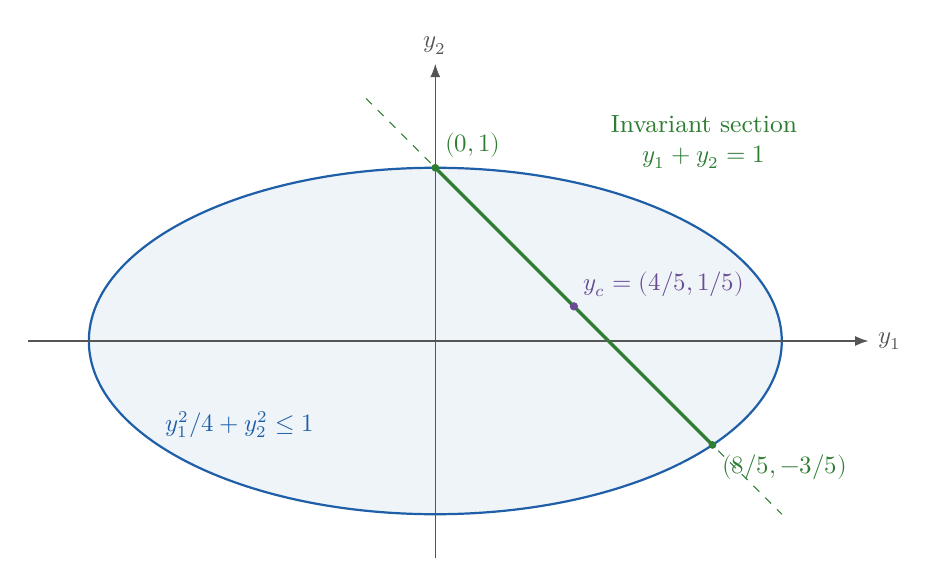
\begin{tikzpicture}[x=2.2cm,y=2.2cm,>=Latex,font=\small]
\fill[elemA!7] (0,0) ellipse (2 and 1);
\draw[elemA,thick] (0,0) ellipse (2 and 1);
\draw[->,frameline] (-2.35,0)--(2.5,0) node[right] {$y_1$};
\draw[->,frameline] (0,-1.25)--(0,1.6) node[above] {$y_2$};
\draw[elemC,dashed] (-.4,1.4)--(2,-1);
\draw[elemC,very thick] (0,1)--(1.6,-.6);
\fill[elemC] (0,1) circle (1.4pt) node[above right] {$(0,1)$};
\fill[elemC] (1.6,-.6) circle (1.4pt) node[below right] {$(8/5,-3/5)$};
\fill[elemD] (.8,.2) circle (1.5pt) node[above right] {$y_c=(4/5,1/5)$};
\node[elemA,align=center] at (-1.13,-.48) {$y_1^2/4+y_2^2\leq1$};
\node[elemC,align=center] at (1.55,1.15) {Invariant section\\$y_1+y_2=1$};
\end{tikzpicture}
\end{document}
